\begin{myblock}{\large Software Packages}

	\begin{figure}[thb!]
		\centering
		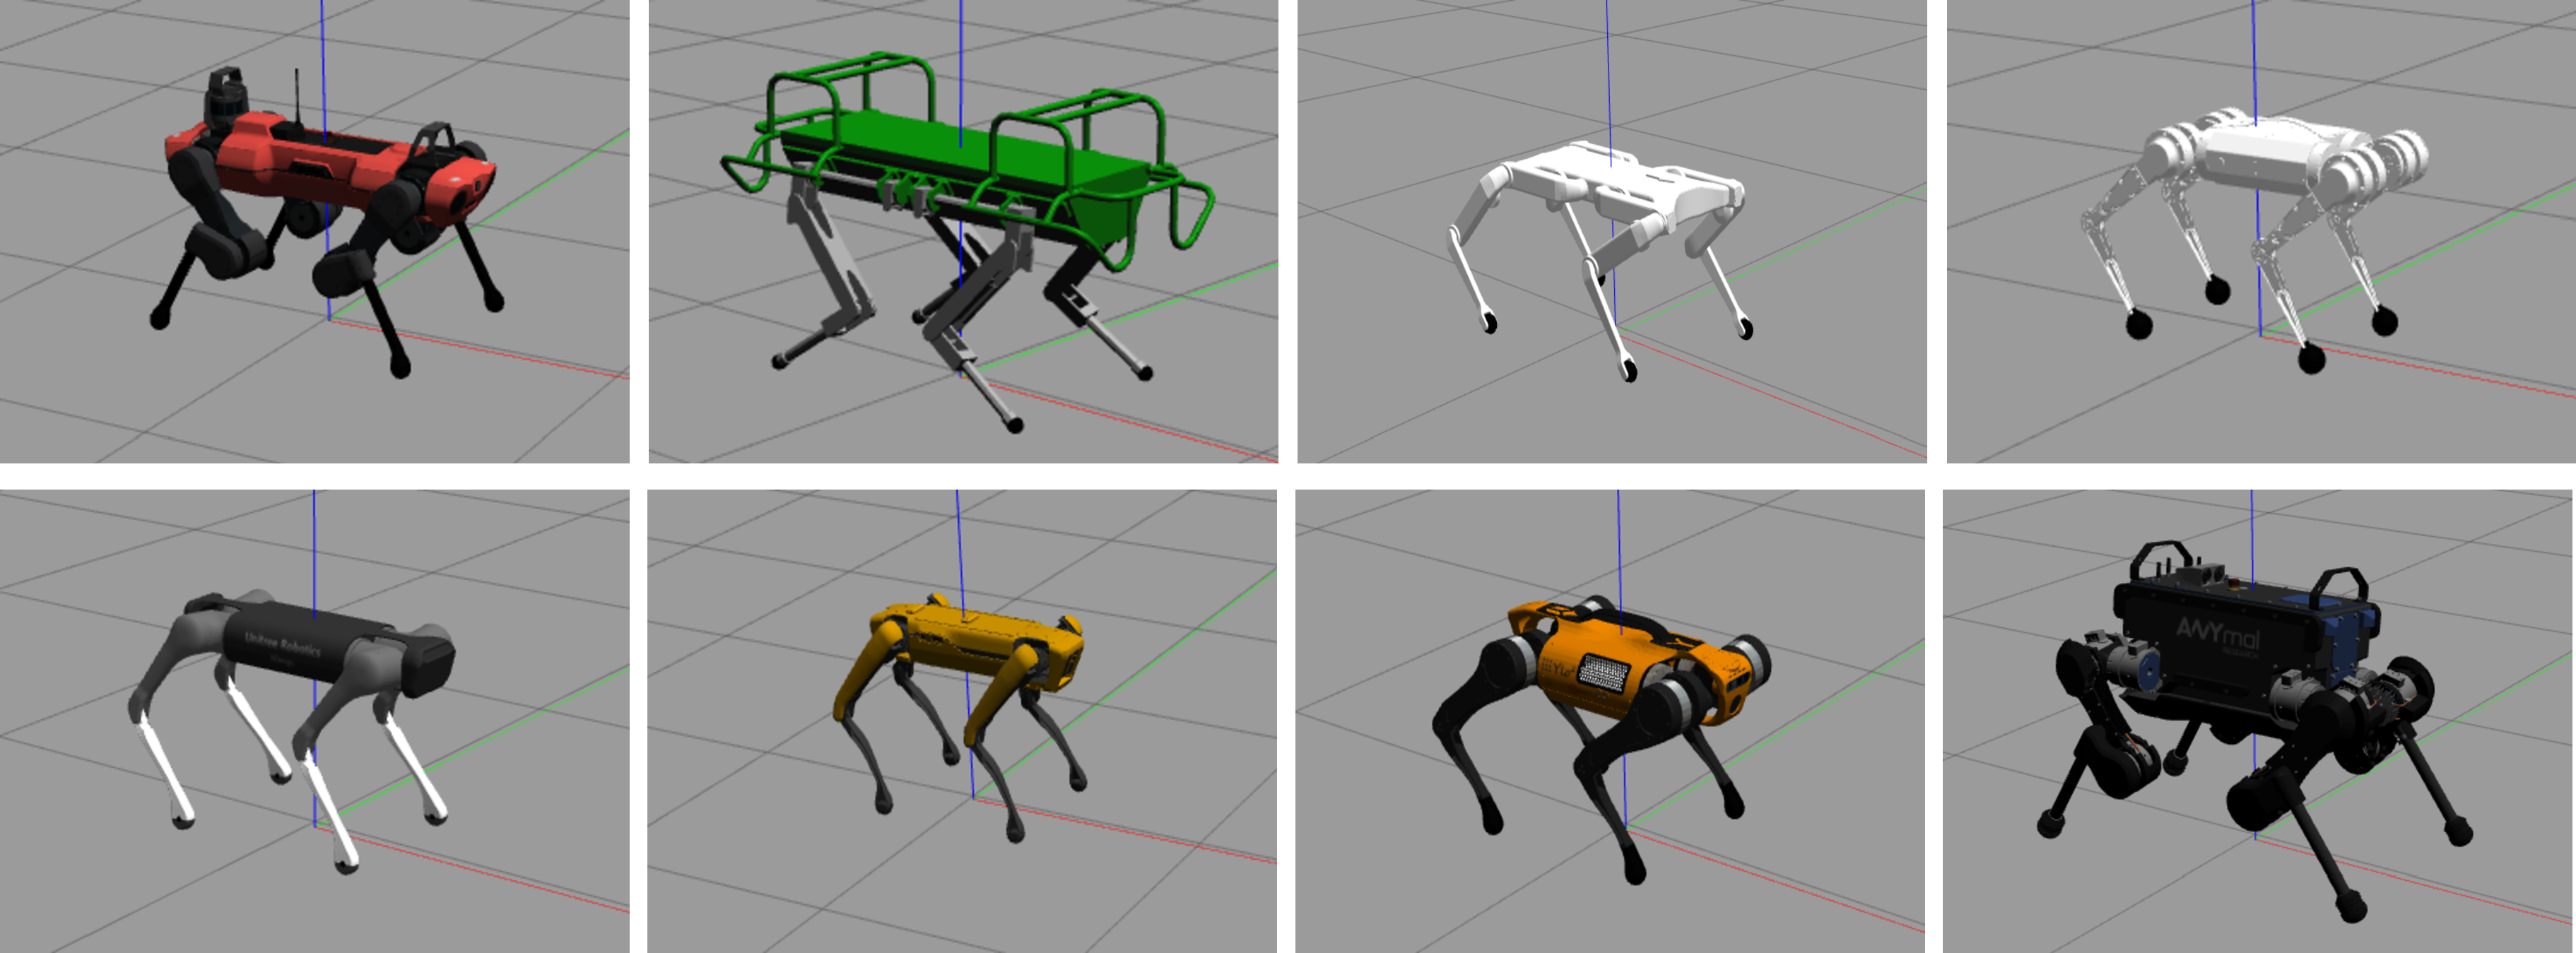
\includegraphics[width=0.8\columnwidth]{images/all_robots.pdf}
		\caption{Robots currently supported in simulation by WoLF. From top-left to bottom-right: AnymalC, HyQ, Solo, Minicheetah, Aliengo, Spot\textsuperscript\textregistered \ , Ylo2, Anymal.}
		\label{fig:robots}
	\end{figure}
	
	The various WoLF packages are hosted on Github. The entry point to set up and run WoLF on any Ubuntu PC is its setup package\footnote{\url{https://github.com/graiola/wolf-setup}}. The other packages are:
	\begin{itemize}
		\item wolf\_descriptions% \footnote{\url{https://github.com/graiola/wolf_descriptions}}
		: it contains robot and sensor descriptions used within the framework (Figure~\ref{fig:robots}). It is possible to use this package to add and try new robots.
		\item wolf\_gazebo\_resources%\footnote{\url{https://github.com/graiola/wolf_gazebo_resources}}
		: it contains Gazebo models and other resources to adapt and create customized simulation environments.
		\item wolf\_hardware\_interface%\footnote{\url{https://github.com/graiola/wolf_hardware_interface}}
		: it implements the hardware interface for ros\_control to be used with WoLF.
		\item wolf\_gazebo\_interface%\footnote{\url{https://github.com/graiola/wolf_gazebo_interface}}
		: This is the Gazebo hardware interface for ros\_control.
		\item wolf\_aliengo\_interface%\footnote{\url{https://github.com/graiola/wolf_aliengo_interface}}
		: Aliengo hardware interface for WoLF. 
		\item wolf\_ylo2\_interface% \footnote{\url{https://github.com/graiola/wolf_ylo2_interface}}
		: Ylo2 hardware interface for WoLF.
		\item wolf\_navigation% \footnote{\url{https://github.com/graiola/wolf_navigation}}
		: This package is used to provide navigation capabilities to WoLF. It integrates and provides several utilities such as odometry computation, way-point definition, and so on.
	\end{itemize}
\end{myblock}	
	
	
\vspace{-20pt}	
\begin{myblock}{\large Applications} 
	%
Applications range from nuclear decommissioning to mining, search \& rescue, inspection, and surveillance. In addition, this technology can be applied to help human workers
in order to reduce labor accidents, as well as in elderly
care and space exploration. The main focus for most end-users is the ability to operate either autonomously or semi-autonomously, through tele-operation.
%	
\begin{figure}[thb!]
	\centering
	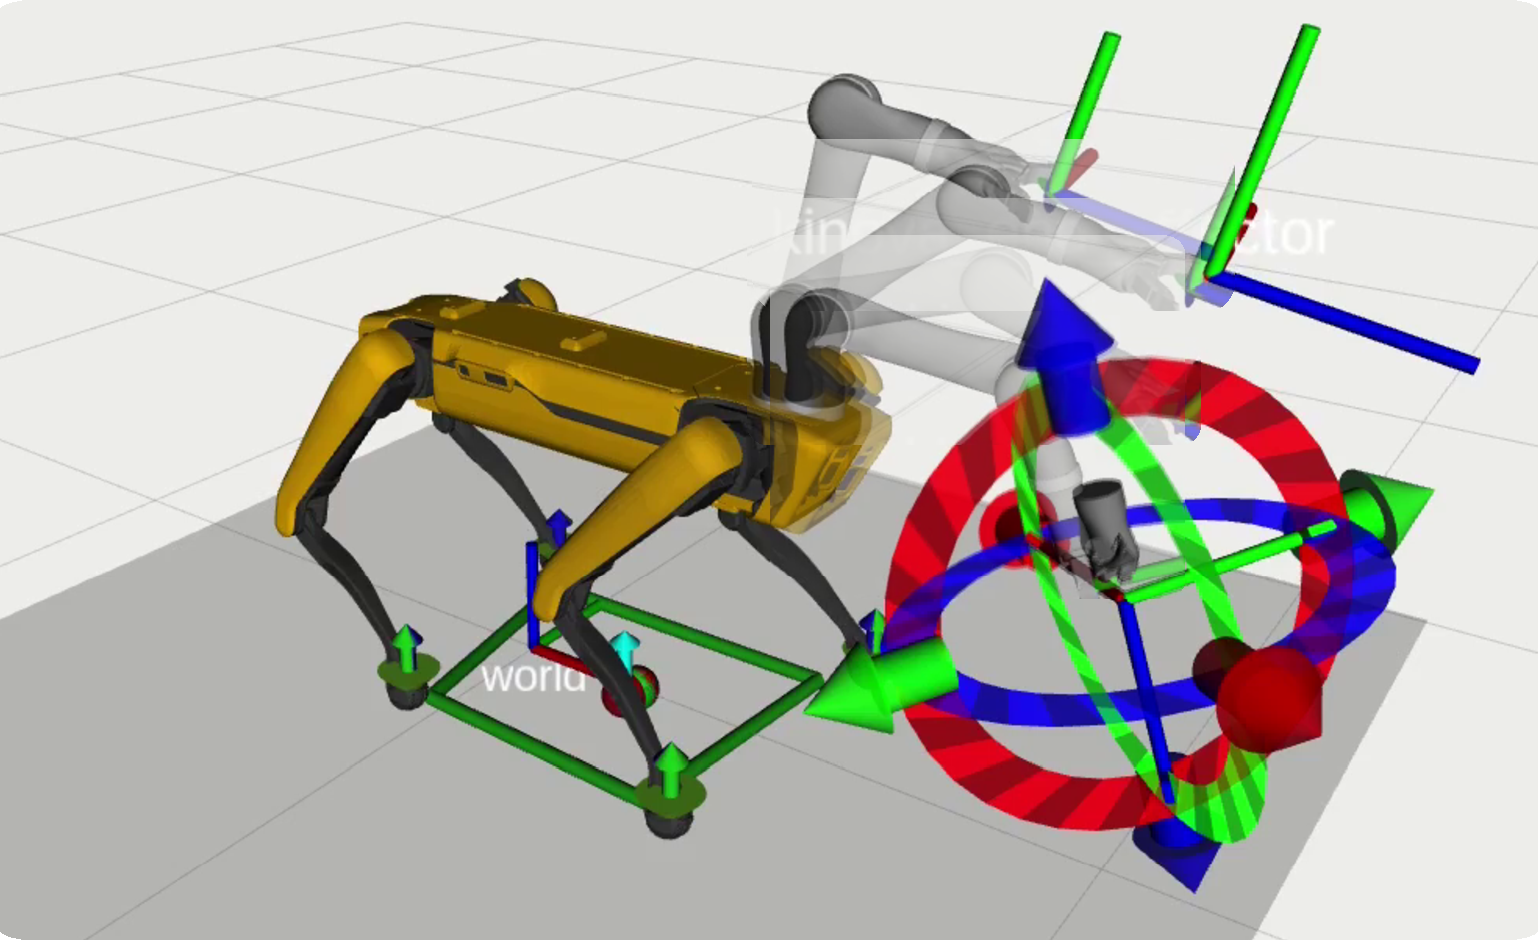
\includegraphics[width=0.5\columnwidth]{images/spot_arm.pdf}
	\caption{Spot\textsuperscript\textregistered \  with a kinova manipulator mounted on its base. WoLF permits to easily combine quadruped platforms with different robotic manipulators. In this example, the kinova end-effector is tele-operated with a ROS interactive marker.}
	\label{fig:spot_arm}
\end{figure}
%
%In this section, we list some of the possible applications of the framework to use cases that are nowadays of increasing interest for the end-users. 
%
\begin{figure}[thb!]
	\centering
	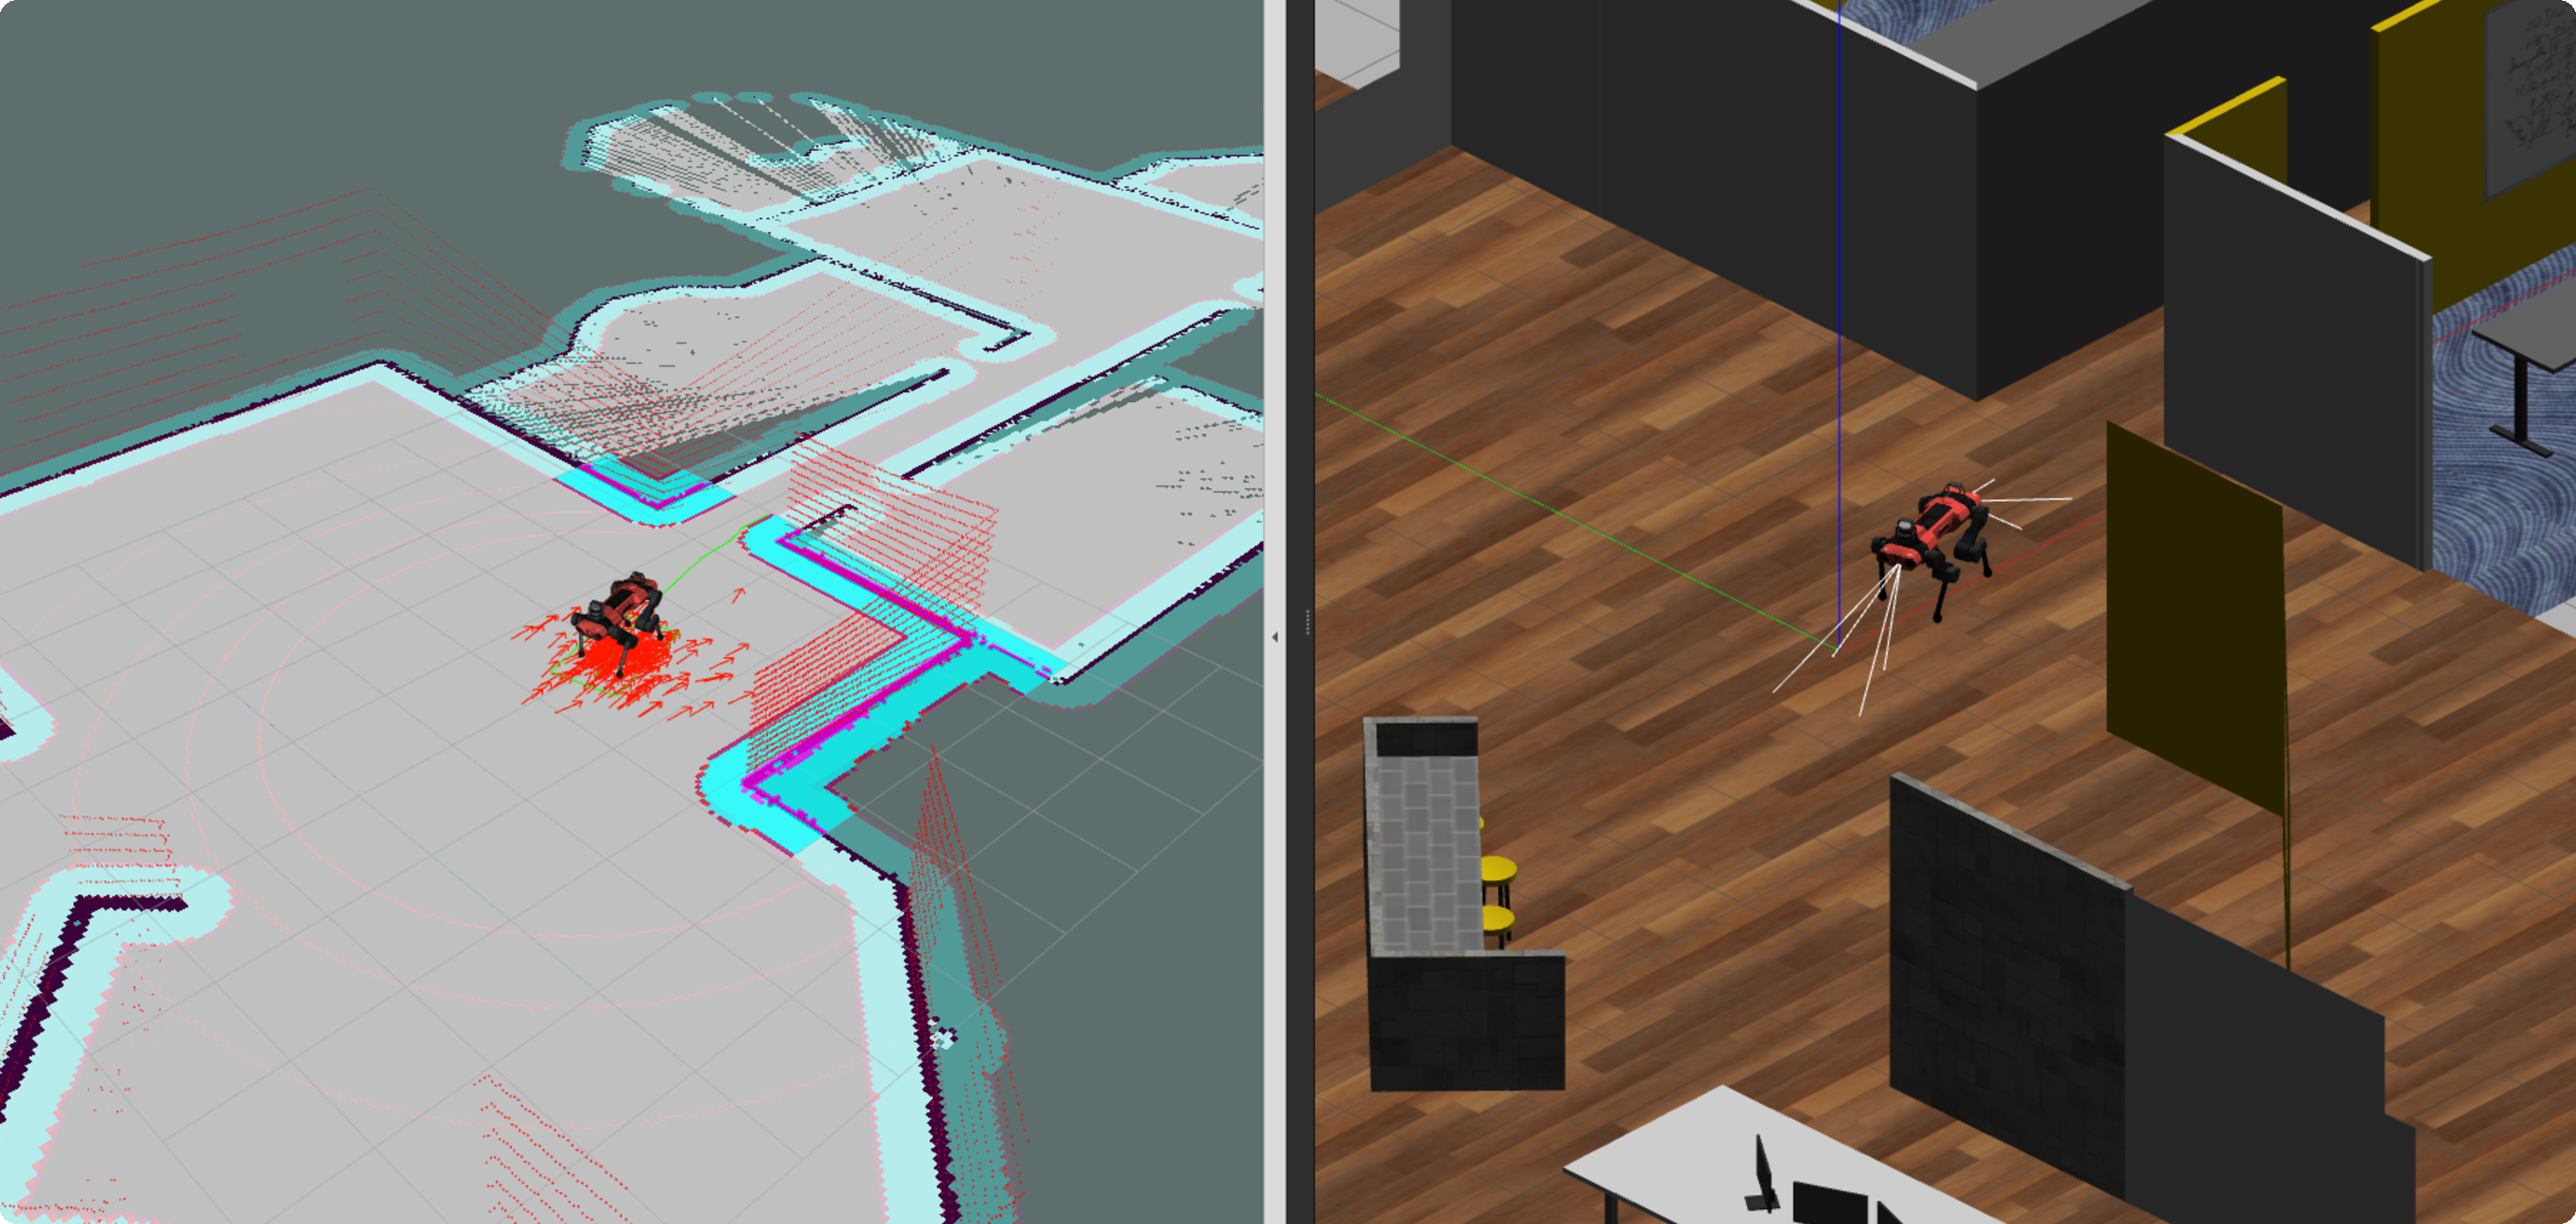
\includegraphics[width=0.5\columnwidth]{images/anymalc_navigation.pdf}
	\caption{AnymalC navigating and reconstructing the map in simulation scenario.}
	\label{fig:anymalc_navigation}
\end{figure}
%
\end{myblock}

%\vspace{-20pt}
\begin{myblock}{{\large Conclusions}}
\begin{itemize}

	\item WoLF provides a plug-and-play software framework easy to tune and adaptable to any quadruped robot without the need for specific knowledge about locomotion or control.
	\item It promote strandardization: use of established robotics tools and technologies such as ROS Gazebo, OpenSoT.
	\item It extend the capabilities of quadrupedal platforms with manipulation and navigation skills.

\end{itemize}
	
\end{myblock} 
